
\begin{figure}[t]
    %\hspace{-10pt}
    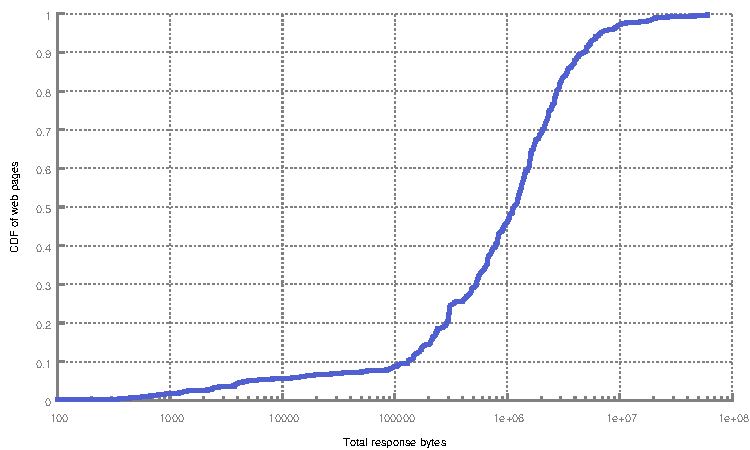
\includegraphics[width=3.25in]{../graphs/total_bytes/total_bytes.pdf}
    \caption[]{\label{fig:total_bytes} Total Bytes.}
\end{figure}

\begin{figure}[t]
    %\hspace{-10pt}
    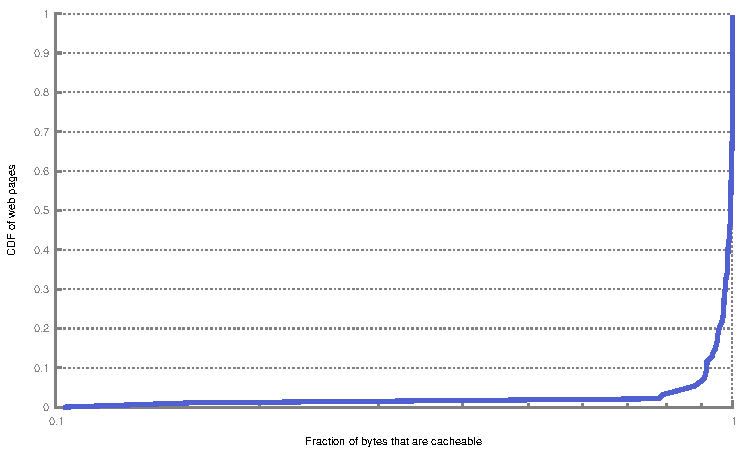
\includegraphics[width=3.25in]{../graphs/cacheable_bytes/cacheable_bytes.pdf}
    \caption[]{\label{fig:cacheable_bytes} Cacheable Bytes.}
\end{figure}

\begin{figure}[t]
    %\hspace{-10pt}
    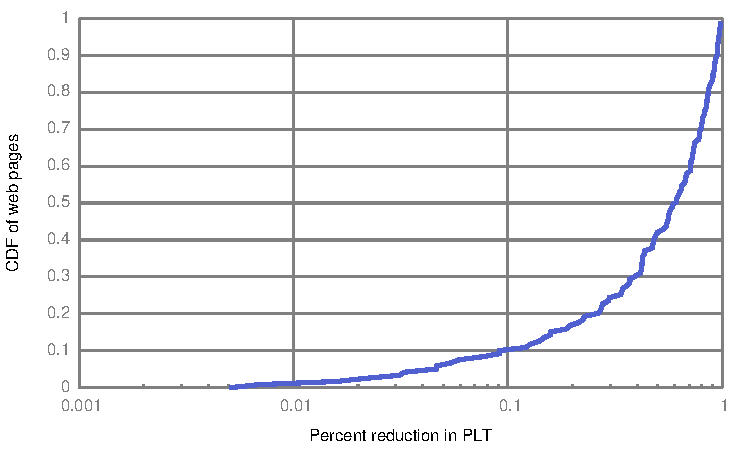
\includegraphics[width=3.25in]{../graphs/percent_plt_reduction/percent_reduction.pdf}
    \caption[]{\label{fig:percent_reduction} Fraction Reduction.}
\end{figure}

\begin{figure}[t]
    %\hspace{-10pt}
    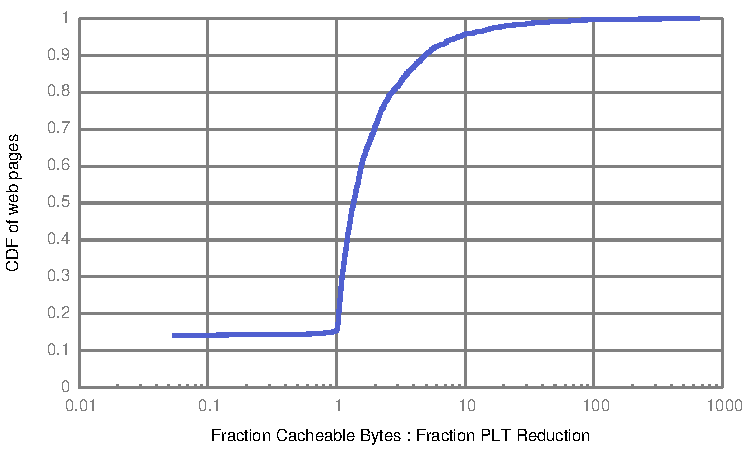
\includegraphics[width=3.25in]{../graphs/ratio_bytes_to_reduction/ratio.pdf}
    \caption[]{\label{fig:ratio} Fraction Cacheable Bytes : Fraction PLT
    Reduction.}
\end{figure}

\begin{figure}[t]
    %\hspace{-10pt}
    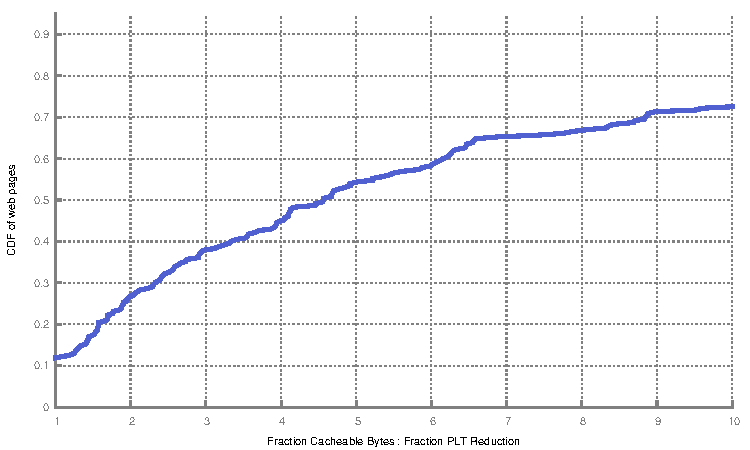
\includegraphics[width=3.25in]{../graphs/ratio_bytes_to_reduction/ratio_linear.pdf}
    \caption[]{\label{fig:ratio_linear} Fraction Cacheable Bytes : Fraction PLT
    Reduction. Linear axis, with datapoints past 95th percentile, and below
    X=1 cut off.}
\end{figure}

Note that all x-axes are in log-scale except for
Figure~\ref{fig:ratio_linear}.

Figure~\ref{fig:ratio} is the most interesting, and requires some pondering.
Datapoints to the left of X=1 indicate that caching yielded a large
bang for its buck, i.e. fraction speedup from perfect caching was greater than fraction of
cacheable bytes. This is about 8\% of the pages. I suspect that this is
largely due to
variation in performance.

At X=1, we see roughly 10\% of pages had PLT improvements commensurate with
fraction of cached byes.

Then right of X=1, the remaining 70ish\% of pages showed that ``a buck's worth
of cache hits amounts to less than a buck's worth of PLT improvement''. It's
hard to see on the logarithmic axis just how many cents of PLT a buck worth of
caching buys. Figure~\ref{fig:ratio_linear} shows us that it's around 75 cents
to the dollar for the 20th through the 40th percentiles. Then it's around 50
cents to the dollar for 40th through the 60th percentiles. After that, the
payoff starts decreasing rapidly for the remaining 40 percentiles.
